\chapter{Introduction}


Humanoid Robotics, Imitation Learning, and Virtual Reality (VR) are some of the most exciting and rapidly developing fields in technology today. It is perhaps no surprise that the marriage of these three technologies can have far-reaching impacts. Using VR, humans can control robots in an immersive simulation, or they can remotely teleoperate robots to perform dangerous tasks. The trajectories from the human demonstrations can then be used to train Imitation Learning policies, which can enable robots to perform the tasks autonomously. While deep Reinforcement Learning methods have been successful in teaching robot to learn from repeated interactions with an environment given a reward function, the sample inefficiency, need for online interactions, and reward engineering efforts make them difficult to implement in a humanoid platform. On the other hand, imitation learning skips over the requirement to create reward functions to shape a behavior and instead shows the robot directly what to do. 

However, due to the complexity of humanoid robots, the lack of large-scale data for training, and the difficulty of creating an intuitive interface for humans to control robots, there has been no research on teaching humanoid robots to perform locomotion and bi-manipulation tasks, as far as I'm aware. There has been work to teach fixed-base robot arms through VR demonstrations \cite{zhang2018deep}, but humanoid robots are significantly more difficult to train due to the need to consider robot dynamics and ground reaction forces. Also, although there is a large body of work on teleoperating humanoids using VR and motion capture devices, I have not found any attempt to use the teleoperation data to train a neural network policy to control the humanoid autonomously. Furthermore, these "telepresence" systems are usually very complicated and require expensive hardware, which makes them unsuitable for scaling up data collection in a distributed manner.

\begin{figure}
	\centering
	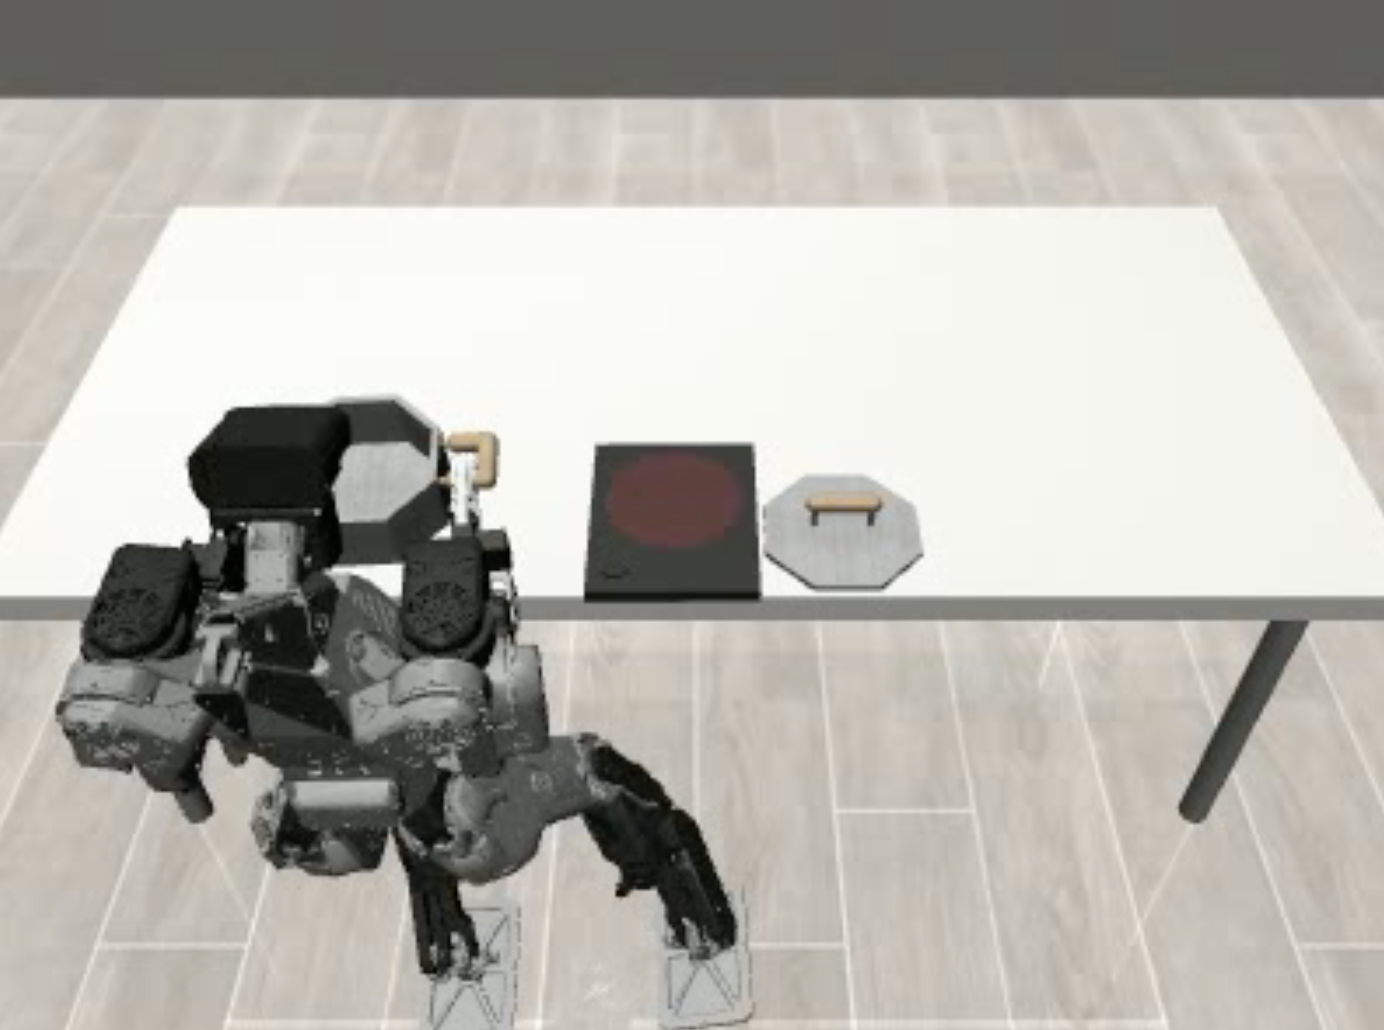
\includegraphics[width=13em]{sim.png}
	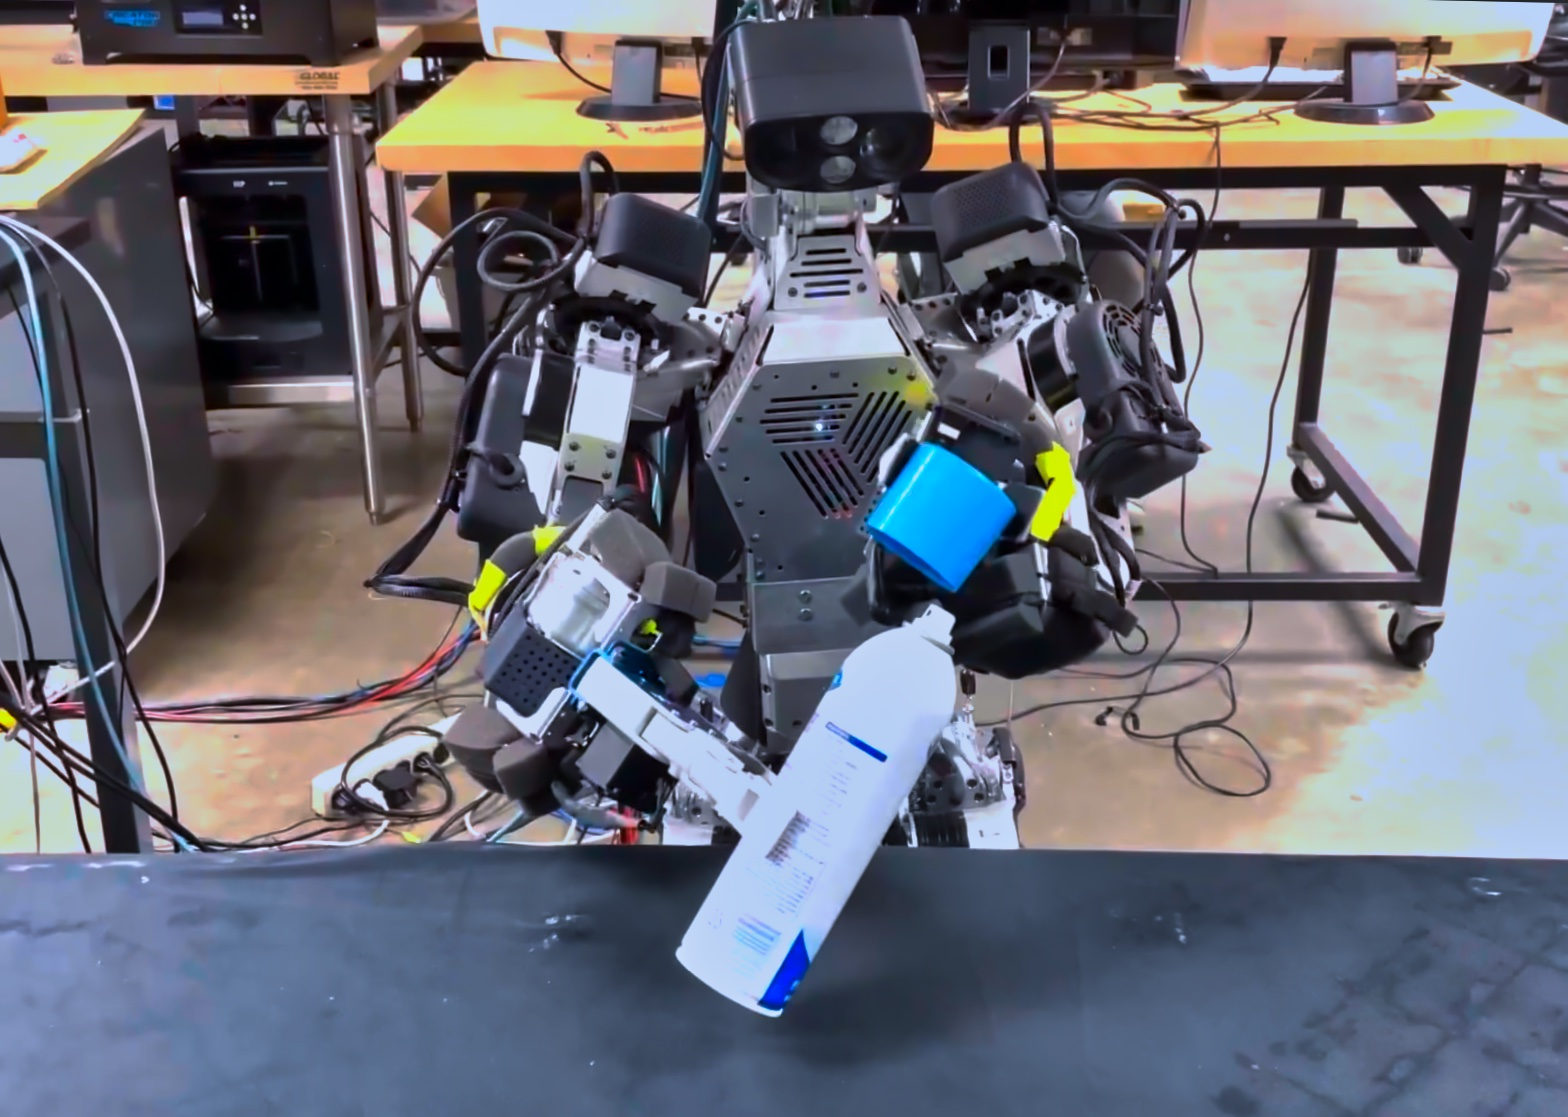
\includegraphics[width=13.6em]{real.jpeg}
	\caption{The proposed interface can be used to teleoperate a simulation environment (left) and a real robot (right).}
    \label{fig:simreal}
\end{figure}

In this thesis, I present a simple VR interface that uses the commonplace Oculus Quest 2 headset. I believe that compared to other humanoid teleoperation systems, the software architecture used in this project is uniquely positioned to be both adaptable to VR games and accessible to the public. Although the interface is simple, it is nonetheless powerful enough to teach a humanoid robot to perform some simple tasks. In simulation, I hypothesize that this setup can be incorporated in VR video games to massively scale up data collection. VR games contain rich interactions with the virtual world, have built-in rewards to label successes and failures, and integrate with powerful physical simulation engines. As a result, they are perfect for collecting human demonstrations to potentially teach humanoids to perform the same tasks in the real world. For example, Cook-Out is a VR game that requires players to cook in a kitchen, which is a valuable skill for humanoids to learn. In addition, on the real-robot side, we could potentially distribute the data collection by letting users with VR headsets control the robot remotely. This is similar to the RoboTurk crowd-sourcing platform for fixed-base arm robots \cite{mandlekar2018roboturk}. I hope that by open-sourcing the teleoperation codebase later this summer, research in humanoid robot learning can be made more accessible. 

To show that we can use the collected demonstrations to train a humanoid to perform simple tasks, we present a hierarchical approach that learns a motion policy from teleoperation demonstrations with an underlying controller. The policy outputs the desired poses of the hands, while the whole-body controller takes care of balancing the robot and tracking the desired trajectory. An overview of this design is presented in Figure \ref{fig:overview}.
\begin{figure}
    \centering
    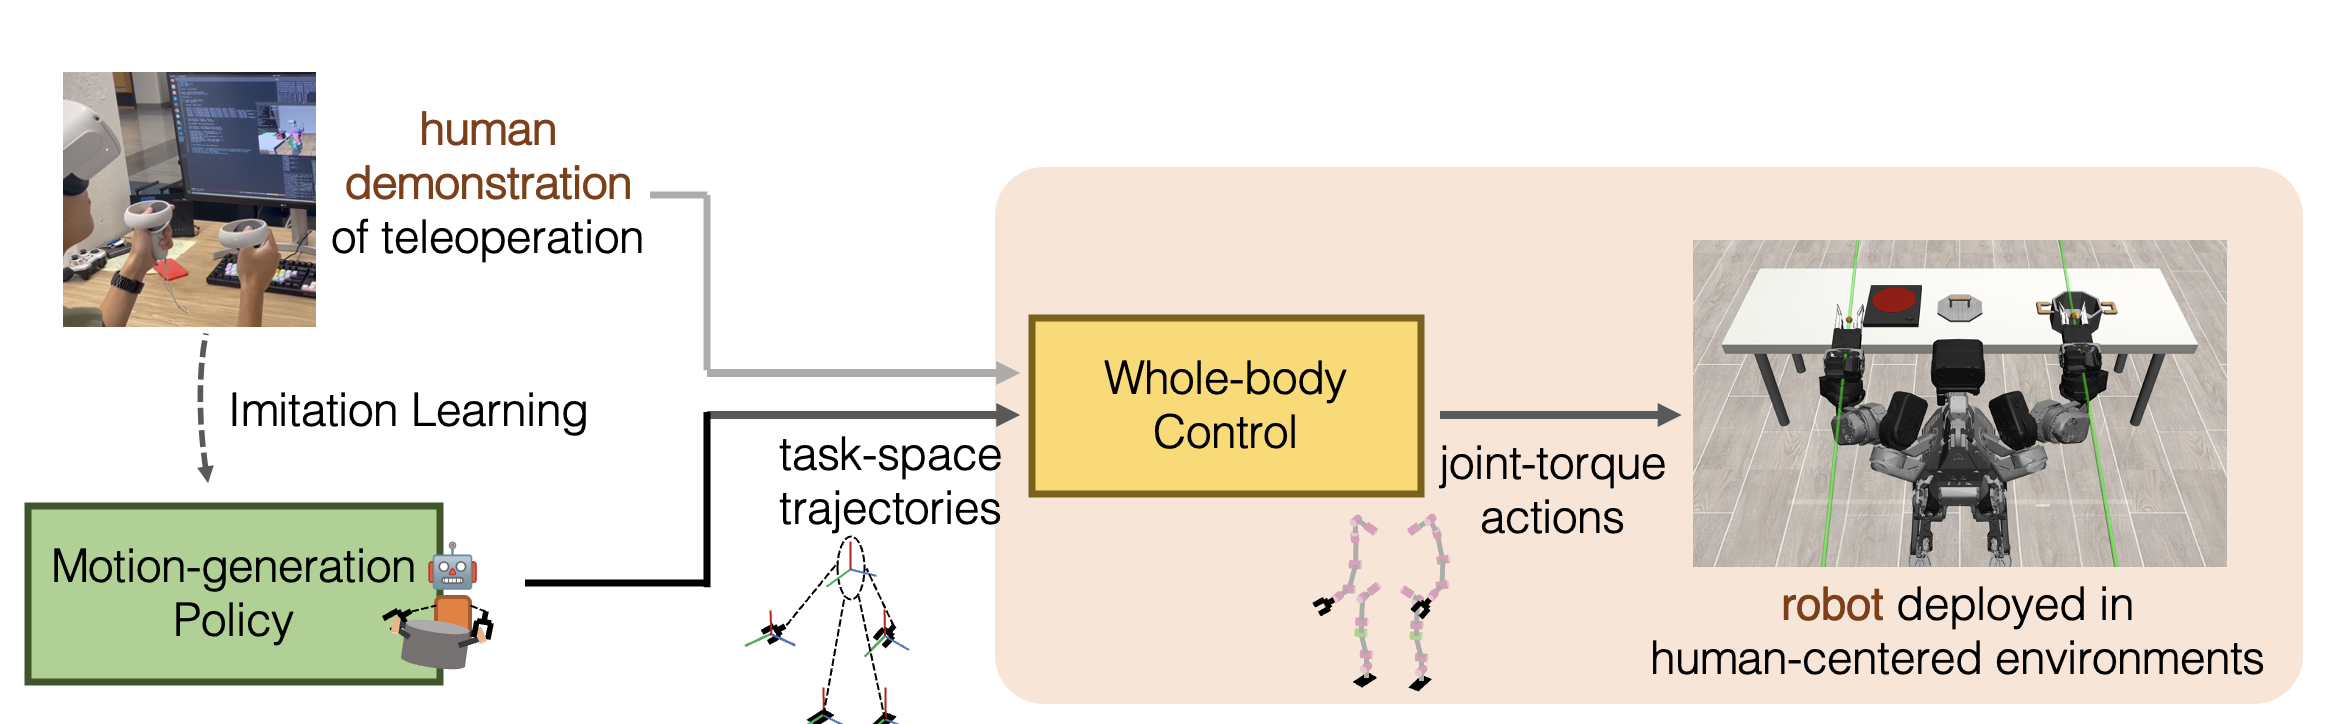
\includegraphics[width=\linewidth]{overview.png}
    \caption{An overview of the hierarchical learning framework used in this work. Diagram credit to Mingyo. First, we get the desired hand trajectories and walking commands from the demonstrator. Second, we send these commands to the whole-body controller to produce joint-torque actions of the robot. Third, a behavior cloning policy is trained to imitate the human demonstrations. }
    \label{fig:overview}
\end{figure}
First, we take advantage of the similar kinematic structures between the robot and demonstrators and collect demonstrations using immersive VR. 
We only record the SE(3) pose of the hands and abstract away the other joint configurations. This lets us easily retarget human motions to the humanoid robot, which has fewer degrees of freedom in the arms. This also makes it easier to learn the motion, since the policy can use the whole-body controller for joint-space controls. Then, we send the desired hand trajectories and walking commands to the whole-body controller to produce joint-torque actions of the robot. The controller prioritizes the robot's stability while tracking the hand and feet trajectories, so it may not track the trajectories perfectly. However, the human demonstrator can adapt to the tracking error by observing the effects of their actions in the VR headset. Finally, a behavior cloning policy is trained to imitate the human demonstrations. The policy needs to learn the state-action distribution of whole-body control behaviors and adapt to it in a closed-loop manner similar to the human. During deployment, the generated trajectories are passed to whole-body control just like during demonstration. The policy achieves reasonable success rate in simple simulation tasks, but it fails for more complex tasks involving manipulation while walking and precise actions. Future research directions to improve the policy will be discussed in the end. 

In the below sections, I go into more details about the motivations for this project.

\section{Humanoid Robots}
Humanoid robots have gained a lot of attention in recent years. After Boston Dynamic's Atlas made headlines by jumping and dancing with human-like dexterity \cite{atlas}, Tesla also entered the market by developing the cheap and mass-producible humanoid named Optimus. If the cost of the robot could be kept below \$20,000 like Elon Musk promised \cite{teslabot}, we would be entering a world where general purpose humanoids could replace humans for unsafe and repetitive tasks. Many startups are also getting a lot of funding recently to pursue humanoid robots. Apptronik is an Austin-based startup that aims to create humanoids that can work alongside people. One of their prototypes, DRACO 3, is the platform used for this thesis.

This interest in humanoids is justified by their versatility and social capabilities. They can be used as personal assistants, as companions for the elderly, as workers in factories, and as first responders in disaster zones. The morphology of humanoids enables them to easily adapt to the human-centered world that we live in. Every tool, every environment, and every task in our society is designed for the human form. It wouldn't make sense to redesign power tools or get rid of stairs for the convenience of robots, so creating robots that can take advantage of the existing infrastructure made for humans is extremely valuable. Also, as humans, it's easier to provide demonstrations to a robot that has a similar form as us, rather than having to train our brain to adapt to the morphology of the robot.

\section {VR Teleoperation Interface}
In order for imitation learning to succeed on robots, high-quality demonstrations are essential. Using a VR interface is desirable since it closes the observation and embodiment gap. Instead of looking at the robot externally, the human will have the same perception as the robot. Instead of having to map the human body's joints to the robot's joints, the human is directly controlling the robot's joints. Because of the human brain's impressive capability to adapt, the demonstrator can quickly learn to treat the arms of the robot as their own arms, and perform tasks intuitively as they do in their own body. Indeed, there are various experiments that shows that humans can start to take ownership of their virtual body, even if the body is very different from their own, if appropriate multisensory correlations are provided \cite{10.3389/fnhum.2015.00141} \cite{10.3389/neuro.09.006.2008}. 

In addition, since humanoid robots have to maintain balance while following hand trajectories, the whole-body controller may fail to track the hand trajectory perfectly. So, in order to move the robot hand to a desired position, one needs to constantly observe the effects of their actions before deciding where to move next. In experiments, we notice that humans are great at adapting to the whole-body control's tracking error in this closed-loop manner. By using the VR interface, we are essentially borrowing the human brain's power to solve the embodiment mismatch issue and perform closed-loop actions. 

\section{Scaling up Demonstration Dataset for Humanoids}

Recently, we have seen the successes of training deep learning algorithms on mind-blowingly huge datasets. For example, GPT-4 \cite{openai2023gpt4} is believed to be trained on most texts on the internet, which enables its scalable transformer architecture to produce human-like texts. The ability of the transformer to scale can also impact the robot learning field, since many transformer architectures for robotics has been proposed with impressive results \cite{zhu2023viola} \cite{jiang2022vima}. Notably, researchers at Google demonstrated that their transformer architecture is able to absorb a large dataset of multi-task demonstrations from different robots and even simulations, and the resulting model is able to generalize to unseen tasks, environments, and objects in a zero-shot manner \cite{brohan2022rt1}. Importantly, they demonstrated that by incorporating simulation data with the real-robot data, not only was the real-robot policy not degraded, but the generalization performance also improved significantly on objects only seen in simulation. This shows that even if the simulation isn't very realistic, the model can still absorb useful information that helps with generalization. The researchers stated that their dataset "consists of over 130k episodes, which contain over 700 tasks, and was collected with a fleet of 13 robots over 17 months." The scale of this dataset is very impressive, but the collection procedure seems very costly, and it is still small in scale compared to the billions of images used to train today's image generation models. In addition, the dataset isn't publicly available, and they are collected on single-arm wheeled robots instead of humanoids. 

So, how can we scale up humanoid demonstration collection in a cheaper manner than investing manpower to collect demonstrations on the real robot? 
One proposal is to learn from the plethora of YouTube videos online. 
For example, \cite{chang2020semantic} shows that by watching YouTube videos of house tours, an off-policy Q-learning algorithm can learn the semantic cues in a human environment to improve navigation efficiency. To make it possible to learn dexterous manipulation skills from YouTube videos, \cite{sivakumar2022robotic} trained a neural network to retarget human finger poses from a video to a robotic hand. 
However, due to the difficulty of inferring 3D poses from video, the lack of proprioceptive view from the eyes of the human, and the ignorance of the person's internal state such as their joint positions, the wealth of information that online videos possess still remain out of reach for practical applications of robot learning. 

Between learning from YouTube videos and collecting demonstrations on the real robot, taking advantage of the rich manipulation data from VR applications might just be practical enough to scale up humanoid data to satiate the appetite of today's deep learning methods. In VR, the human sees exactly what the robot sees, the hand poses are measured precisely by the headset and controllers, and the simulated robot provides full access to its internal states. As realistic simulation games such as Microsoft Flight Simulator rise up in popularity, we are presented with a valuable opportunity to collect high-quality human hand trajectories at scale for robot-learning research. This is not unreasonable since Meta is most likely already collecting information about the users' surroundings and actions for targeted ads \cite{oculus-privacy}.
